% SiMate

\chapter{SiMate}

\section{Elicitação de Requisitos}

Tomando como base o contexto do sistema, os requisitos foram elicitados e, nesta seção, estão divididos em regras de negócios, requisitos funcionais e requisitos não funcionais.

Para facilitar o entendimento e evitar a repetição desnecessária, a sigla CRUD (acrónimo de Create, Read, Update e Delete na língua Inglesa) será usada como representação das ações de criação, visualização, edição e exclusão do modelo associado.

\subsection{Regras de Negócio} \label{subsec:regras_de_negocio}

Regras de negócio declaram e refletem as regras do produto, definindo assim as instruções de como o sistema irá atingir o seu objetivo obedecendo a políticas internas, o processo definido e as determinações básicas de conduta. 

Nesta subseção, restrições, validações, comportamentos, exceções e os demais elementos que compõem o conjunto de instruções que o sistema a ser desenvolvido deve contemplar serão definidos.

\begin{enumerate}[label=\textbf{RN\protect\twodigits{\theenumi}}, leftmargin=2cm]
	\item \label{rn:administrador} Todos os usuários que possuírem o papel de Administrador devem ter completo acesso a todas as funcionalidades do sistema. \\
		\textbf{Prioridade:} Alta \\
		\textbf{Depende de:} Nenhum

	\item \label{rn:artefato_na_etapa} Após entrar em um fluxo, o material de aula ou prova (artefato) só pode participar de uma etapa por vez. Estando em uma etapa, somente os usuários que possuem o papel responsável pela etapa em questão podem agir sobre o artefato, fazendo alterações, avaliações e o repassando para uma das próximas etapas disponíveis. Essa regra não vale para usuários com papel de administrador (ver \hyperref[rn:administrador]{\ref{rn:administrador}}). \\
		\textbf{Prioridade:} Média \\
		\textbf{Depende de:} \hyperref[rn:administrador]{\ref{rn:administrador}}

	\item \label{rn:etapa_inicial_e_final_do_fluxo} O fluxo do material pode ser representado por um grafo de arestas bidirecionas, dessa forma, não há definição do vértice (etapa) inicial e final, logo é necessário que o fluxo guarde explicitamente o nome dessas duas etapas. \\
		\textbf{Prioridade:} Alta \\
		\textbf{Depende de:} Nenhum

\end{enumerate}

\subsection{Requisitos Funcionais}
		
\begin{enumerate}[label=\textbf{RF\protect\twodigits{\theenumi}}, leftmargin=2cm]

	\item \label{rf:papeis} O sistema deve permitir o gerenciamento (CRUD) dos papéis. Cada papel representa uma função que pode ser exercida por um ou mais usuários. As determinações dessas funções podem ser entendidas na subseção \hyperref[subsec:regras_de_negocio]{Regras de Negócio} \\
		\textbf{Prioridade:} Alta \\
		\textbf{Depende de:} \hyperref[rn:administrador]{\ref{rn:administrador}}

	\item \label{rf:usuarios} O sistema deve permitir, além das ações de CRUD, o login e logout dos usuários. \\
		\textbf{Prioridade:} Alta \\
		\textbf{Depende de:} Nenhum

	\item \label{rf:etapas} O sistema deve permitir o gerenciamento (CRUD) das etapas. A etapa representa o estado em que um material de aula ou prova (artefato) pode estar dentro de um fluxo. Se um material de aula é enviado de um professor para a revisão didática, por exemplo, podemos dizer que o artefato em questão está na etapa de transição didática e que os responsáveis pela revisão são os usuários que possuem o papel de equipe de transição didática.  \\
		\textbf{Prioridade:} Alta \\
		\textbf{Depende de:} \hyperref[rn:artefato_na_etapa]{\ref{rn:artefato_na_etapa}}

	\item \label{rf:fluxos} O sistema deve permitir o gerenciamento (CRUD) dos fluxos. Para melhor entendimento, pode-se pensar no fluxo como um grafo de arestas bidirecionais, onde cada vértice é uma etapa e as arestas são possibilidades de transição das etapas do material. \\ 
	Por exemplo, estando um material de aula na etapa de transição didática (vértice) ela pode seguir para a correção do professor (aresta ligando etapa de transição didática e etapa de correção do professor) ou pode ir para a revisão LP/ABNT (aresta ligando etapa de transição didática à etapa de revisão LP/ABNT). Como a representação de grafo aqui definida não sugere etapa inicial e final, o fluxo deve guardar explicitamente a determinação dessas duas etapas (ver \hyperref[rn:etapa_inicial_e_final_do_fluxo]{\ref{rn:etapa_inicial_e_final_do_fluxo}}). \\
		\textbf{Prioridade:} Alta \\
		\textbf{Depende de:} \hyperref[rf:etapas]{\ref{rf:etapas}}

	\item \label{rf:artefatos} O sistema deve permitir o gerenciamento (CRUD) de artefatos. O artefato pode assumir um dos seguintes tipos: aula ou prova. Ele tem uma data de entrega e pertence a uma oferta. Além disso, cada artefato possui n versões, sendo n definido pelo número de etapas que o artefato passou dentro do fluxo da sua oferta. Cada versão é caracterizada por ter autor, data de criação, arquivo e mensagem. \\
		\textbf{Prioridade:} Alta \\
		\textbf{Depende de:} \hyperref[rf:ofertas]{\ref{rf:ofertas}} e \hyperref[rf:fluxos]{\ref{rf:fluxos}}
				
	\item \label{rf:modulos} O sistema deve permitir o gerenciamento (CRUD) dos módulos. Cada módulo representa um espaço de tempo de um determinado ano com datas de início e fim bem definidas. Os módulos participam de um semestre, ou seja, cada módulo possui associação com um semestre do ano letivo. \\
		\textbf{Prioridade:} Alta \\
		\textbf{Depende de:} Nenhum

	\item \label{rf:disciplinas} O sistema deve permitir o gerenciamento (CRUD) de disciplinas. Disciplinas representam áreas do conhecimento que serão posteriormente usadas para criar as ofertas. \\
		\textbf{Prioridade:} Alta \\
		\textbf{Depende de:} Nenhum
		
	\item \label{rf:ofertas} O sistema deve permitir o gerenciamento (CRUD) de ofertas. Cada oferta designa, de fato, o conjunto de aulas e provas (artefatos) de uma área de conhecimento (disciplina) que acontecem em um determinado período de um semestre (módulo). \\
		\textbf{Prioridade:} Alta \\
		\textbf{Depende de:} \hyperref[rf:modulos]{\ref{rf:modulos}}, \hyperref[rf:disciplinas]{\ref{rf:disciplinas}}, \hyperref[rf:fluxos]{\ref{rf:fluxos}} e \hyperref[rf:artefatos]{\ref{rf:artefatos}}
		
	\item \label{rf:fluxo} O sistema deve permitir a criação dos materiais. Essa criação pode ser definida como um conjunto de passos que adicionam, validam e corrigem o material, permitindo assim que ele esteja pronto para ser usado ao final do fluxo. \\
	O passo introdutório do processo de elaboração da aula/prova deve ser dado pelo usuário responsável pela etapa inicial, permitindo assim que as outras etapas aconteçam até que o material chegue a etapa conclusiva. \\	
	\textbf{Prioridade:} Alta \\
	\textbf{Depende de:} \hyperref[rn:artefato_na_etapa]{\ref{rn:artefato_na_etapa}}, \hyperref[rn:etapa_inicial_e_final_do_fluxo]{\ref{rn:etapa_inicial_e_final_do_fluxo}}, \hyperref[rf:papeis]{\ref{rf:papeis}}, \hyperref[rf:usuarios]{\ref{rf:usuarios}}, \hyperref[rf:etapas]{\ref{rf:etapas}}, \hyperref[rf:fluxos]{\ref{rf:fluxos}}, \hyperref[rf:artefatos]{\ref{rf:artefatos}}, \hyperref[rf:modulos]{\ref{rf:modulos}}, \hyperref[rf:disciplinas]{\ref{rf:disciplinas}} e \hyperref[rf:ofertas]{\ref{rf:ofertas}}
	
\end{enumerate}

\subsection{Requisitos Não-Funcionais}

\begin{enumerate}[label=\textbf{RNF\protect\twodigits{\theenumi}}, leftmargin=2cm]

	\item \label{rf:papeis} O sistema deve estar disponível 24 horas/dia e 7 dias/semana, afim de garantir que as metas estabelecidas para criação dos materiais não sejam quebradas por indisponibilidade da aplicação. \\
		\textbf{Categoria:} Disponibilidade e Confiabilidade \\
		\textbf{Escopo:} Sistema \\
		\textbf{Prioridade:} Alta \\
		\textbf{Depende de:} Nenhum

	\item \label{rf:papeis} O sistema deve lidar com os vários níveis de acesso dos usuários restringindo a interação com os conteúdos a eles associados. \\
		\textbf{Categoria:} Segurança de Acesso \\
		\textbf{Escopo:} Funcionalidade \\
		\textbf{Prioridade:} Alta \\
		\textbf{Depende de:} Nenhum

	\item \label{rf:papeis} O sistema deve trazer uma interface amigável, simples, rápida e eficiente. \\
		\textbf{Categoria:} Usabilidade, Atratividade e Desempenho \\
		\textbf{Escopo:} Sistema \\
		\textbf{Prioridade:} Alta \\
		\textbf{Depende de:} Nenhum

	\item \label{rf:papeis} Para garantir a fácil manutenção pela equipe a qual será entregue o sistema após o desenvolvimento, esse deve ser implementado utilizando a linguagem de programação JAVA. \\
		\textbf{Categoria:} Implementação \\
		\textbf{Escopo:} Sistema \\
		\textbf{Prioridade:} Alta \\
		\textbf{Depende de:} Nenhum

	\item \label{rf:papeis} Para garantir a fácil manutenção pela equipe a qual será entregue o sistema após o desenvolvimento, esse deve ser implementado utilizando a linguagem de programação JAVA. \\
		\textbf{Categoria:} Implementação \\
		\textbf{Escopo:} Sistema \\
		\textbf{Prioridade:} Alta \\
		\textbf{Depende de:} Nenhum

\end{enumerate}

\section{Especificação de Casos de Uso}

Nesta seção serão especificados as unidades funcionais que representam as necessidades principais do sistema. No primeiro tópico, os atores participantes dessas funcionalidades serão conceituados e, após isso, será feito o detalhamento dos casos de uso.

\subsection{Atores}

\subsubsection{Administrador}

O ator Administrador representa a pessoa que tem poder total sobre o sistema. Nenhuma funcionalidade é restringida a esse tipo de usuário.

\subsubsection{Setor de Materiais}

No sistema, o usuário possuidor do papel de Setor de Materiais é responsável principalmente por gerir a execução do fluxo, permitindo assim auditoria e intervenção no processo.

\subsubsection{Genérico}

O ator Genérico existe para representar usuários como o professor e os membros das demais equipes no sistema. O principal objetivo desse tipo de usuário é participar do fluxo de materiais contribuindo para que o material seja desenvolvido.

\subsection{Casos de Uso}
     
\begin{enumerate}[label=\textbf{UC01}, leftmargin=2cm]
	\item \textbf{Criar Etapa} \\
	A etapa representa um possível passo em qualquer fluxo, dessa forma, cada etapa pode participar de diversos fluxos ao mesmo tempo, sendo a ela atribuído somente nome, responsáveis e descrição. \\
	\begin{minipage}[c]{10cm}
	    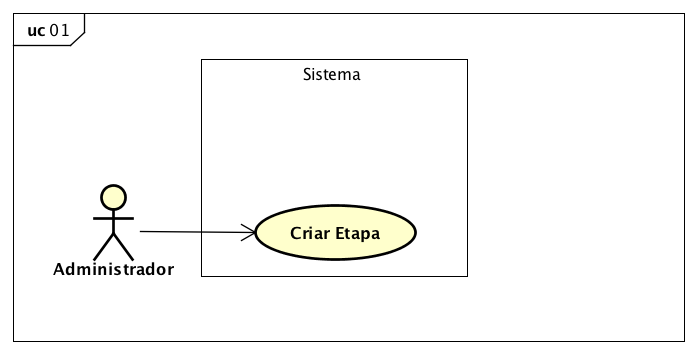
\includegraphics[width=10cm]{Imagens/UC_CriarEtapa.png}
	    \captionof{figure}{Diagrama do Caso de Uso Criar Etapa}
		\label{fig:uc_criar_fluxo}
	\end{minipage} \\

	\begin{enumerate}[label=, leftmargin=0cm]
		\item \textbf{Atores} \\
		Administrador
		\item \textbf{Precondições}
			\begin{enumerate}[label=\arabic*.]
				\item Usuário estar logado no sistema.
			\end{enumerate}
		\item \textbf{Fluxo Básico}
			\begin{enumerate}[label=\arabic*.]
				\item Usuário solicita o formulário de criação de etapa.
				\item O sistema exibe formulário onde o usuário deve preencher o nome da etapa, os responsáveis pela execução da etapa e uma descrição
				\item Usuário preenche formulário.
				\item O sistema valida os dados e informa que o fluxo com salvo com sucesso.
			\end{enumerate}
		\item \textbf{Pós-condições}
			\begin{enumerate}[label=\arabic*.]
				\item Uma nova etapa foi criada e pode ser visualizado, editado, excluído ter passos do fluxo associados a ela.
			\end{enumerate}
	\end{enumerate}
	 
\end{enumerate}

\begin{enumerate}[label=\textbf{U02}, leftmargin=2cm]
	\item \textbf{Criar Fluxo} \\
	Este caso de de uso detalha a elaboração do fluxo e suas etapas. No sistema, um fluxo criado representa o passo-a-passo para a criação dos materiais associados. \\
	\begin{minipage}[c]{10cm}
	    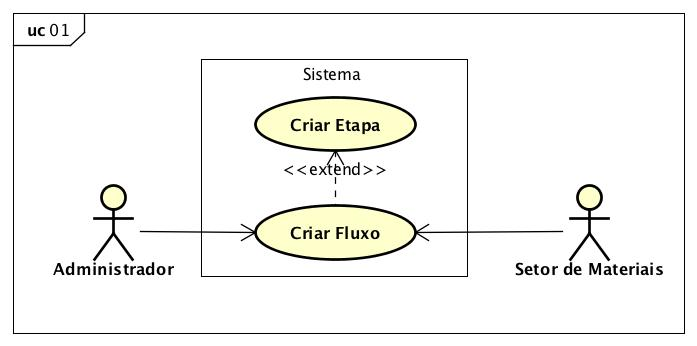
\includegraphics[width=10cm]{Imagens/UC_CriarFluxo.jpg}
	    \captionof{figure}{Diagrama do Caso de Uso Criar Fluxo}
		\label{fig:uc_criar_fluxo}
	\end{minipage} \\

	\begin{enumerate}[label=, leftmargin=0cm]
		\item \textbf{Atores} \\
		Administrador e Setor de Materiais
		\item \textbf{Precondições}
			\begin{enumerate}[label=\arabic*.]
				\item Usuário estar logado no sistema.
			\end{enumerate}
		\item \textbf{Fluxo Básico}
			\begin{enumerate}[label=\arabic*.]
				\item Usuário solicita o formulário de criação de fluxo.
				\item O sistema exibe formulário onde o usuário deve preencher o nome do fluxo, definir os possíveis caminhos que o fluxo pode tomar a partir das etapas e, por último, definir etapa final e inicial.
				\item Usuário preenche formulário.
				\item O sistema valida os dados e informa que o fluxo com salvo com sucesso.
			\end{enumerate}
		\item \textbf{Fluxo Alternativo A}
			\begin{enumerate}[label=\arabic*.]
				\item No passo 2 do Fluxo Básico, o sistema não retorna etapas anteriormente criadas e/ou o usuário de tipo Administrador decide criar uma nova etapa para ser usada no fluxo. 
				\item Usuário solicita formulário de criação de etapa.
				\item Sistema exibe formulário onde o usuário deve preencher o nome da etapa, os responsáveis e uma descricão.
				\item Usuário preenche o formulário.
				\item Sistema valida, informa que a etapa foi criada e retorna ao passo 2 do Fluxo Básico.
			\end{enumerate}
		\item \textbf{Fluxo Alternativo B}
			\begin{enumerate}[label=\arabic*.]
				\item No passo 4 do Fluxo Básico, o sistema invalida o formulário por falta de informação e/ou os passos do fluxo não estão consistentes.
				\item O sistema informa os erros presentes no formulário e solicita que o usuário corrija os erros.
				\item Volta ao passo 3 do Fluxo Básico.
			\end{enumerate}
		\item \textbf{Pós-condições}
			\begin{enumerate}[label=\arabic*.]
				\item Um novo fluxo foi criado e pode ser visualizado, editado, excluído e associado à materiais.
			\end{enumerate}
	\end{enumerate}
	 
\end{enumerate}

\begin{enumerate}[label=\textbf{UC03}, leftmargin=2cm]
	\item \textbf{Criar Material} \\
	Este caso de de uso detalha o processo de criação do material. Para elaboração do material, um fluxo bem definido e consistente deve ser associado.  \\
	\begin{minipage}[c]{10cm}
	    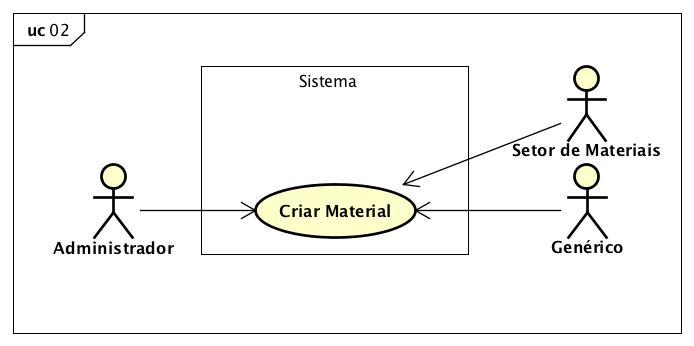
\includegraphics[width=10cm]{Imagens/UC_CriarMaterial.jpg}
	    \captionof{figure}{Diagrama do Caso de Uso Criar Material}
		\label{fig:uc_criar_material}
	\end{minipage} \\

	\begin{enumerate}[label=, leftmargin=0cm]
		\item \textbf{Atores} \\
		Administrador, Setor de Materiais e Genérico.
		\item \textbf{Precondições}
			\begin{enumerate}[label=\arabic*.]
				\item Existir oferta cadastrada com módulo e disciplina.
				\item Existir artefato de aula ou prova relacionado com a oferta.
				\item Existir um fluxo associado ao artefato.
				\item Usuários responsáveis pelas etapas do fluxo estarem logados no sistema.
			\end{enumerate}
		\item \textbf{Fluxo Básico}
			\begin{enumerate}[label=\arabic*.]
				\item Usuário solicita visualização da oferta.
				\item Sistema exibe dados da oferta com todos os artefatos (aula ou prova).
				\item Usuário seleciona artefato que deseja dar início ao processo de criação do material.
				\item Sistema exibe formulário de criação do material com campos para carregamento do arquivo, mensagem e possíveis próximas etapas para as quais esse material pode seguir.
				\item Usuário preenche o formulário, carrega o arquivo e define qual o próximo passo do fluxo.
				\item Sistema recebe os dados, informa ao usuário que o material foi submetido.
				\item Sistema notifica responsáveis pela etapa atual do material e aguarda ação.
				\item Usuário responsável pela etapa atual solicita visualização do material.
				\item Sistema exibe informações do material atual permitindo que o usuário baixe o arquivo.
				\item Usuário solicita criação de nova versão do material atual.
				\item Sistema mostra formulário de criação de nova versão do material atual com campos para carregamento do arquivo, mensagem e possíveis próximas etapas para as quais esse material pode seguir.
				\item Usuário preenche o formulário, carrega o arquivo e define qual o próximo passo do fluxo.
				\item Volta ao passo 6 e repete até que o material chegue à etapa final do fluxo.
				\item Sistema sinaliza que o fluxo do artefato foi completado e que o material está pronto.
			\end{enumerate}
		\item \textbf{Fluxo Alternativo A}
			\begin{enumerate}[label=\arabic*.]
				\item Ao fim do passo 2 do Fluxo básico, um usuário com papel de Administrador decide interver no fluxo e move o material para alguma etapa que não é necessariamente uma das disponíveis a partir da etapa atual.
				\item O fluxo retorna ao passo 13 do Fluxo Básico.
			\end{enumerate}
		\item \textbf{Pós-condições}
			\begin{enumerate}[label=\arabic*.]
				\item O estado de feito é atribuído ao artefato do material.
				\item Há um material pronto e disponível.
			\end{enumerate}
	\end{enumerate}
	 
\end{enumerate}


\section{Projeto de Interface}

Baseando-se nos requisitos elicitados, o projeto de interface foi realizado e os protótipos que serão apresentados a seguir, apesar de se tratarem de \textit{wireframes}, já trazem uma preocupação com a intuitividade e usabilidade do sistema.

O primeiro \textit{wireframe} (Figura \hyperref[fig:pi_tela_inicial]{\ref{fig:pi_tela_inicial}}) demonstra a tela inicial, que deve ser apresentada logo após o login do usuário. Nela, estão organizados alguns elementos como um espaço para alertas de materiais com o prazo emergencial, outro para últimas mensagens recebidas e os fluxos de trabalho ativos. Nesse último, cada bloco representa um fluxo de material cujo produto está na fase que o usuário atual é responsável por contribuir.

\vspace{5mm}
\begin{minipage}[c]{\textwidth}
    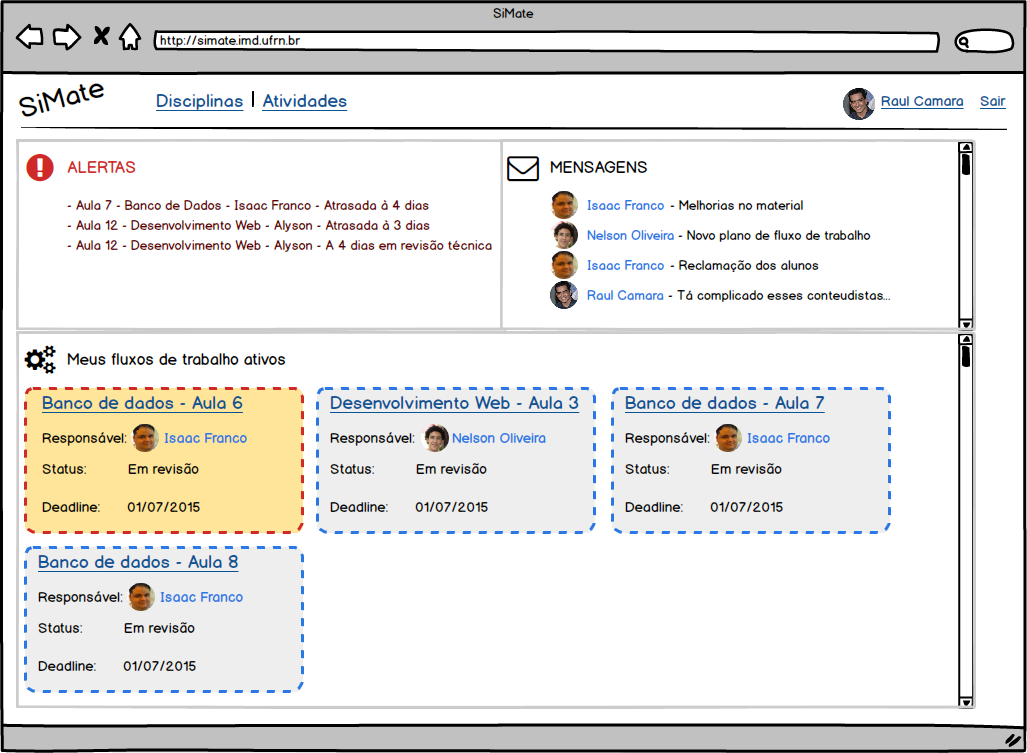
\includegraphics[width=15cm]{Imagens/SiMateTelas/Index.png}
    \captionof{figure}{Tela Inicial}
	\label{fig:pi_tela_inicial}
\end{minipage} \\

Através da barra de navegação do sistema, é possível visualizar as ofertas (representada por disciplinas) do usuário. Essa visualização é apresentada através da grade da Figura \hyperref[fig:pi_grade_disciplinas]{\ref{fig:pi_grade_disciplinas}}.

\vspace{5mm}
\begin{minipage}[c]{\textwidth}
    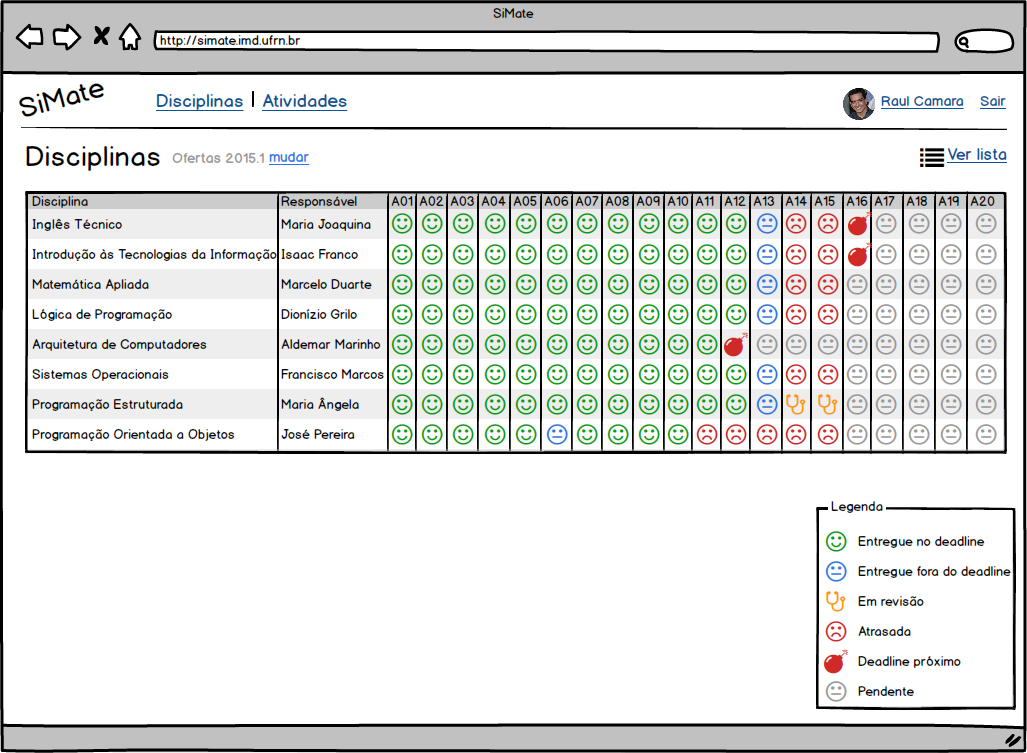
\includegraphics[width=15cm]{Imagens/SiMateTelas/GradeDisciplinas.png}
    \captionof{figure}{Tela de Listagem das Ofertas}
	\label{fig:pi_grade_disciplinas}
\end{minipage} \\

É possível notar que a grade de disciplinas possui uma coluna para responsável, esse é o usuário/equipe que deve dar início ao fluxo de criação do material, e colunas para os artefatos de aulas e provas. Cada artefato possui um estado que pode ser entendido através da legenda no canto inferior direito.

Na próxima tela (Figura \hyperref[fig:pi_artefato_detalhe]{\ref{fig:pi_artefato_detalhe}})), o fluxo do material é mostrado como os detalhes do artefato. 

\vspace{5mm}
\begin{minipage}[c]{\textwidth}
    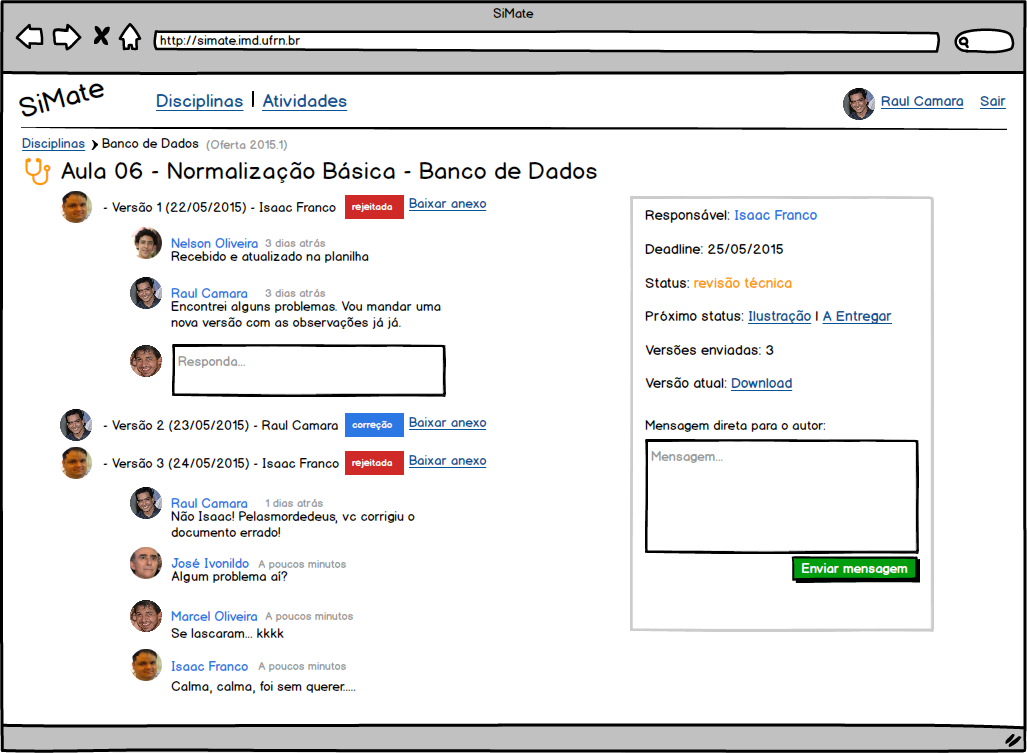
\includegraphics[width=15cm]{Imagens/SiMateTelas/ArtefatoDetalhe.png}
    \captionof{figure}{Tela de Detalhe do Artefato}
	\label{fig:pi_artefato_detalhe}
\end{minipage} \\

Cada versão do material na tela acima registra uma contribuição dentro do fluxo, uma passagem de etapa/passo. É nessa tela que a gerência do setor de materiais poderá entender de forma fácil e prática como anda o processo, podendo assim baixar todas as versões do produtos, analisá-las e interagir com os envolvidos através de comentários. Caso seja necessário que o usuário envie uma nova revisão do material, é possível fazê-lo através do formulário presente no lado direito da tela e este será adicionado ao fim da listagem de versões como esperado.

\section{Arquitetura}

A arquitetura de implementação do projeto se baseia na usada pelo núcleo de desenvolvimento do Instituto Metrópole Digital e pode ser visualizada na figura abaixo.

\vspace{5mm}
\begin{minipage}[c]{\textwidth}
	\centering
    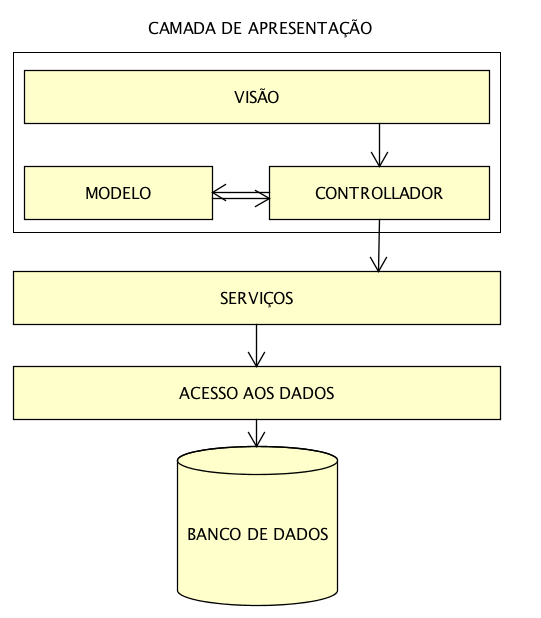
\includegraphics[width=10cm]{Imagens/Arquitetura.png}
    \captionof{figure}{Arquitetura Simplificada do SiMate}
	\label{fig:arq}
\end{minipage} \\

Na Figura \hyperref[fig:arq]{\ref{fig:arq}}, o primeira caixa representa a camada de apresentação no padrão MVC (Modelo - Visão - Controlador) que é um padrão de arquitetura de software onde a Visão representa as telas de interação e as saídas de dados, o modelo representa as regras de negócio e o controlador é o mediador que recebe as entradas através da visão e os converte em comandos gerando ou não uma saída pro usuário. Após isso temos a camada de serviços que oferece as ações disponíveis para manipulação de dados, ações essas que são executadas na camada de acesso aos dados.
